
%
%%%%%%%%%%%%%%%%%%%%%%%%%%%%%%%%%%%%%%%%%%%%%%%%%%%%%%%%%%%%%%%%%%%%%%%%%%%%%%%
% The LHC
%%%%%%%%%%%%%%%%%%%%%%%%%%%%%%%%%%%%%%%%%%%%%%%%%%%%%%%%%%%%%%%%%%%%%%%%%%%%%%%
%
\chapter{The ATLAS detector at the LHC}

\section{The Large Hadron Collider}


The Large Hadron Collider  (LHC)~\cite{Breskin:1244506} is a proton-proton ($pp$) synchrotron located in the previous Large Electron Positron (LEP) collider tunnel at CERN Laboratory, just outside the city of Geneva (Switzerland), approximately 100~m underground. It is designed to collide bunches of up to $\sim 10^{11}$ protons every 25~ns at a center-of-mass energy of 14~TeV (seven times the 2~TeV reached by the Tevatron accelerator at Fermilab Laboratory, in Chicago). During 2011 the LHC operated at a lower collision rate and lower energy (more details will be given in the paragraphs below).

The experiments analyzing the collisions produced by the LHC are distributed around the 27~km ring at the various interaction points. The ATLAS experiment is located at Point 1, which is closest to the main CERN site. Point 5 houses the other general purpose detector, CMS. ALICE and LHCb experiments are located at Point 2 and Point 8, respectively. The former is designed to investigate heavy ion collisions; the latter, to investigate rare decays of b-mesons. The layout of these four experiments along the LHC ring is shown in Fig.~\ref{fig:LHC1}.

\begin{figure}[htbp]
  \begin{center}
      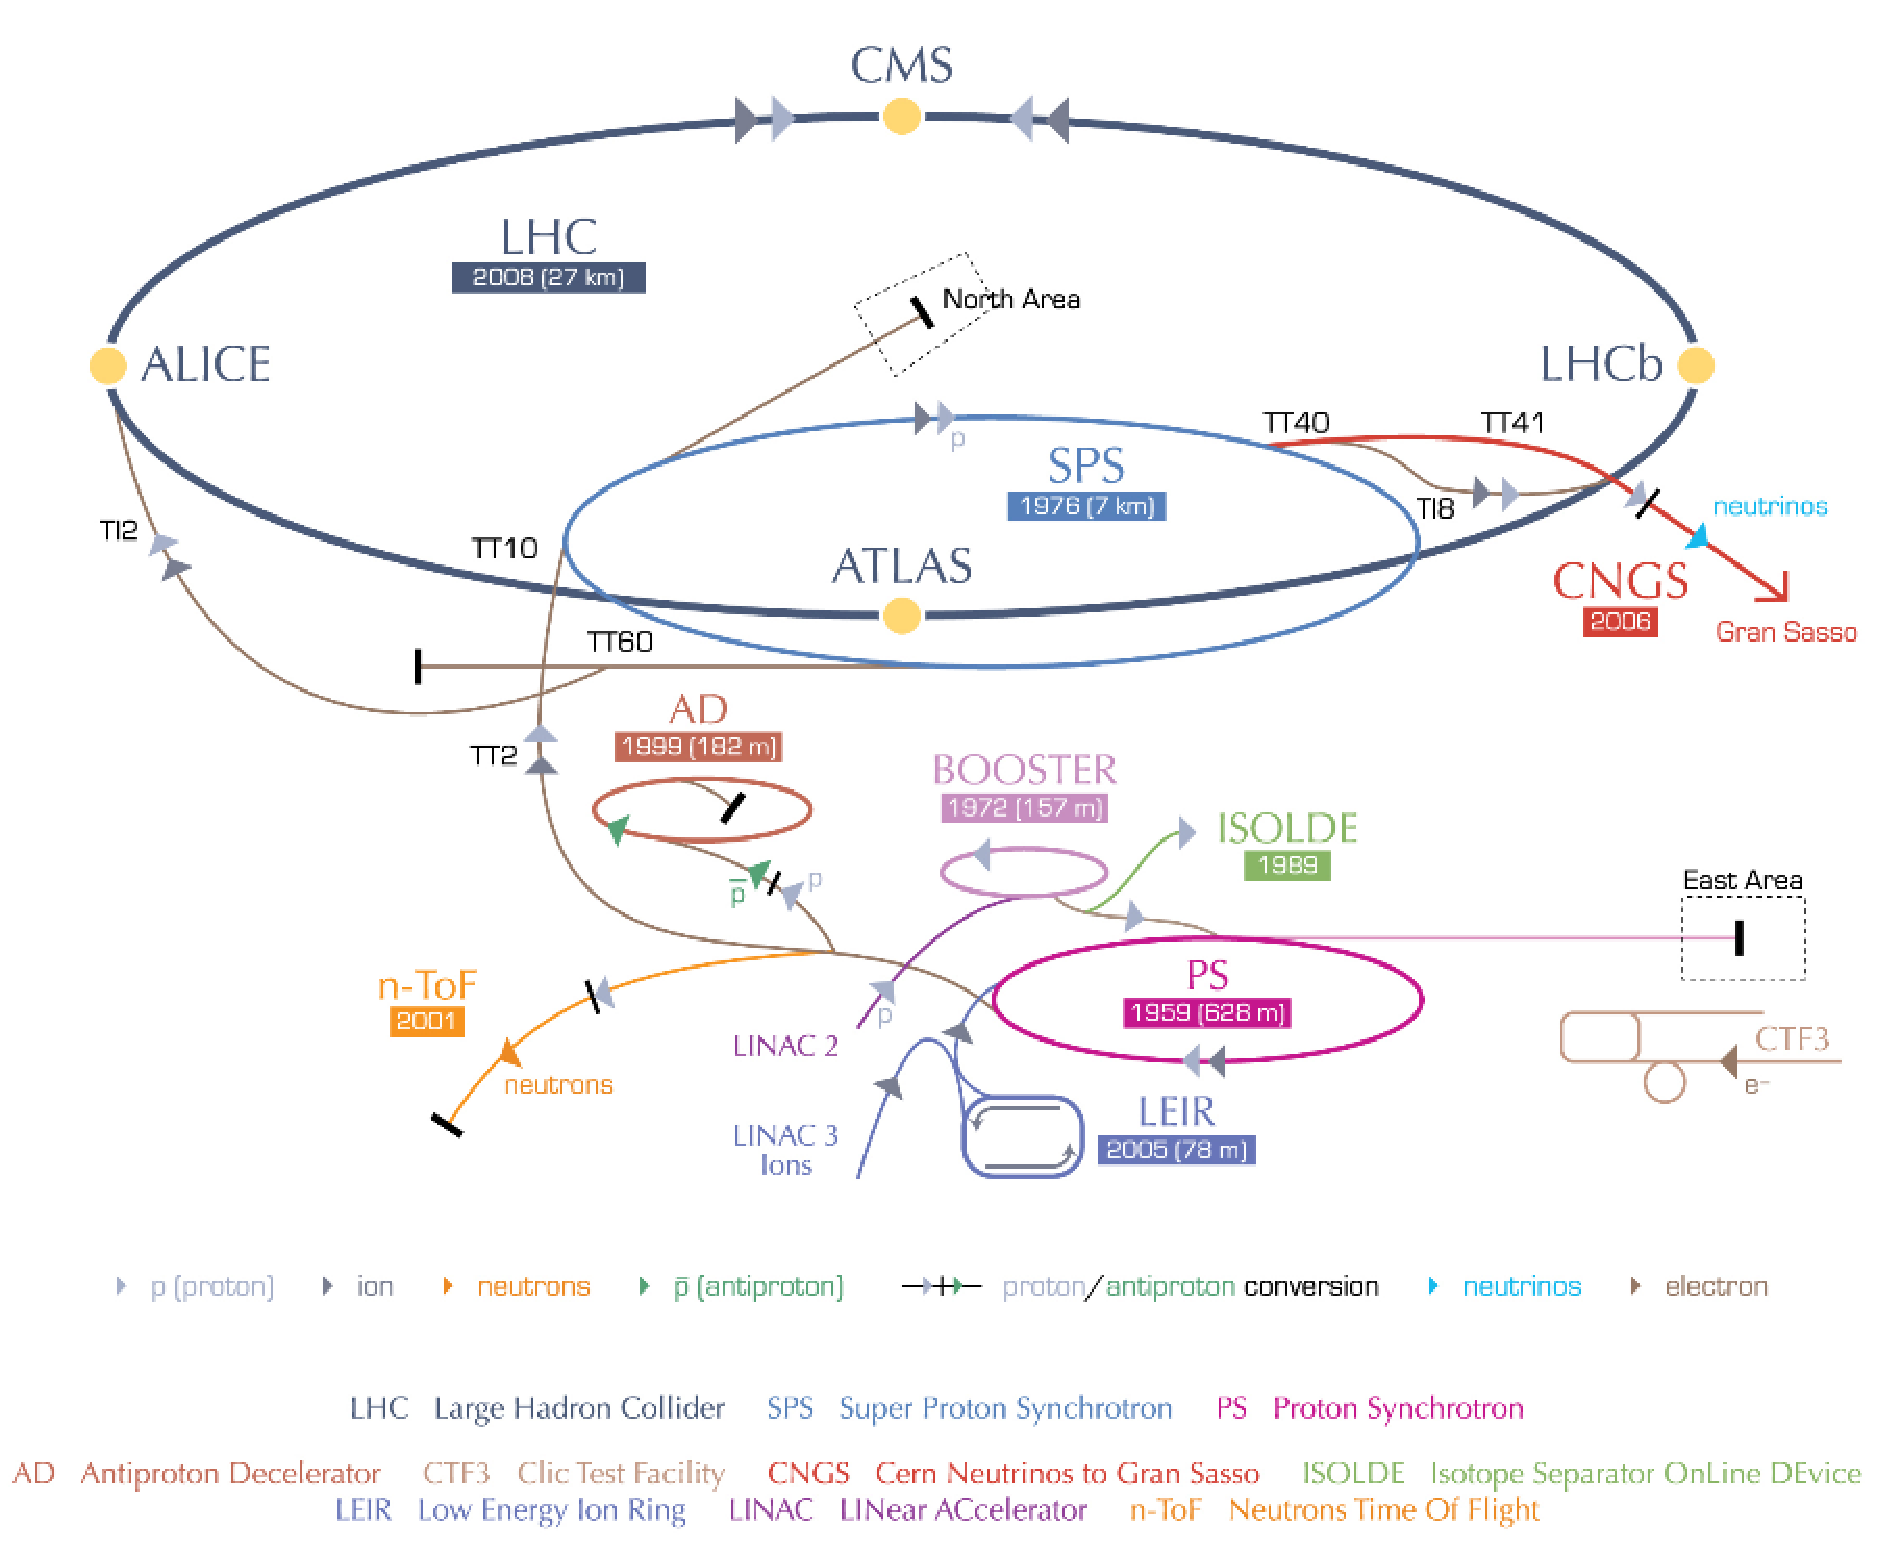
\includegraphics[width=1\textwidth]{Fig2/CERNacceleratorcomplexCut.pdf}
    \caption{The CERN accelerator complex, showing the injection system, along with each component’s date of construction, and the placement of the four main experiments.}
    \label{fig:LHC1}
  \end{center}
\end{figure}

%Proton beams are formed before insertion into the main LHC ring using a series of smaller accelerators, as also shown in Figure 3.1. In order to attain the desired high proton beam energy, the entire accelerator chain uses radio-frequency (RF) acceleration. In RF acceleration, particles travel through a series of time-varying electrical fields. Particles that enter with the correct phase are accelerated along their direction of motion, while those with the incorrect phase are decelerated. The result of a sequence of RF accelerations is several bunches of protons, each traveling with the desired energy. It is important to note that the phrase “LHC beams” in fact refers to many bunches of protons separated by some uniform distance.

%The bunch structure of a modern accelerator is a direct consequence of the radio frequency (RF) acceleration scheme. Protons can only be accelerated when the RF field has the correct orientation when particles pass through an accelerating cavity, which happens at well specified moments during an RF cycle.

Proton beams are formed before insertion into the main LHC ring using a succession of smaller machines with increasingly  higher energies, as shown in Fig.~\ref{fig:LHC1}. The chain begins as protons are injected into the PS Booster (PSB) at an energy of 50~MeV from Linac2. The booster accelerates them to 1.4~GeV. The beam is then fed to the Proton Synchroton (PS) where it is accelerated to 25~GeV. At desin strength, the bunch structure, known as a bunch train, contains 72 bunches of protons upon entry to the Super Proton Synchrotron (SPS). The SPS accumulates up to four fills of 72 bunches from the PS and accelerates them to 450~GeV, with a bunch spacing of $\sim$~25~ns. They are finally transferred to the LHC (both in a clockwise and an anticlockwise direction) where they are accelerated for 20 minutes to their nominal energy of 7 TeV. Beams will circulate for many hours inside the LHC beam pipes under normal operating conditions.

%Increasing the number of bunches is one of the ways to increase luminosity in a machine. 
%The bunch spacing of 25 ns corresponds to a frequency of 40 MHz, which implies that bunches should pass each of the collision points in the LHC 40 million times a second. 
%When the bunches cross, there will be a maximum of about 20 collisions

BLABLABLA
Maybe here a description of the magnetic field?
BLABLABLA
BLABLABLA

The rate of events produced by the colliding beams depends on the luminosity of the collisions, which is a measure of the number of events per second per unit cross section, typically measured in units cm$^2$s$^{-1}$. The number of events of a particular process, then, is given by the product of the integrated luminosity, $\int dt L$, and the cross section of the process, $\sigma_{event}$.  The integrated luminosities are typically quoted in units of inverse picobarns, pb$^{-1}$ = 10$^{-36}$cm$^{2}$. In order to measure processes with very little cross sections a very high luminosity is required. 

The delivered luminosity can be written as~\cite{ATLAS-CONF-2011-116}:

\begin{equation} 
\mbox{ {\it L }} = \frac{n_b f_r n_1 n_2 }{2\pi \Sigma_x \Sigma_y}
\label{eqn:lumi}
\end{equation} 
where n$_b$ is the number of colliding bunch pairs,  n$_1$ and n$_2$ are the bunch populations (protons per bunch) in beam 1 and beam 2 respectively (together forming the bunch charged product), $f_r$ is the machine revolution frequency, and $\Sigma_x$ and $\Sigma_y$ are the width and the height of the proton beams. %characterize the horizontal and vertical profiles of the colliding beams. 
The number of protons per bunch, the number of bunches per beam, and the revolution frequency are all set by the beam operators. The widths of the proton beams can be measured in a process known as a Van der Meer ($vdM$) scan~\cite{vanderMeer:296752}. In a $vdM$ scan, the beams are separated by steps of a known distance. The collision rate is measured as a function of this separation, and the width of a gaussian fit to the distributions yields the width of the beams in the direction of the separation. 





%------------------------------------------------------------------------
%\subsection{Luminosity and pile-up}\label{sec:lumiintro}
%------------------------------------------------------------------------





%
%%%%%%%%%%%%%%%%%%%%%%%%%%%%%%%%%%%%%%%%%%%%%%%%%%%%%%%%%%%%%%%%%%%%%%%%%%%%%%%
% ATLAS
%%%%%%%%%%%%%%%%%%%%%%%%%%%%%%%%%%%%%%%%%%%%%%%%%%%%%%%%%%%%%%%%%%%%%%%%%%%%%%%
%
\section{The ATLAS Detector}

%------------------------------------------------------------------------
\subsection{Detector overview}\label{sec:atlassummary}
%------------------------------------------------------------------------
El dectector ATLAS, ac\'ronimo para A Toroidal LHC Apparatus, fue dise\~nado para estudiar la f\'isica de colisiones \emph{p-p} en el LHC. Todo el detector est\'a contenido en un cilindro de aproximadamente 44 metros de largo por 22 metros de di\'ametro y pesa unas 7000 toneladas\cite{TDR}.  Presenta una estructura tipo cebolla, pudiendo separarse en tres sistemas comenzando desde el punto de interacci\'on: el detector interno, los calor\'imetros y el sistema de muones (figura \ref{fig:ATLAS}) . Cada parte se divide a su vez en m\'as capas. Las part\'iculas emergentes atraviesan primero el detector interno, donde se reconstruye la trayectoria de las part\'iculas cargadas. En el calor\'imetro todas las part\'iculas, con excepci\'on de muones y neutrinos, depositan toda su energ\'ia y se detienen. Los muones interact\'uan electromagn\'eticamente al igual que los electrones, pero al ser mucho m\'as masivos que \'estos no emiten radiaci\'on de frenado y logran atravesar el calor\'imetro dando se\~nal en el sistema de detecci\'on de muones. ATLAS cuenta adem\'as con un sistema de imanes que provee de un campo magn\'etico que curva las trayectorias de las part\'iculas cargadas que atraviesan el detector interno y el espectr\'ometro de muones, permitiendo medir su momento.

   Todos los detectores de ATLAS, as\'i como el sistema de imanes, se componen de un barril central y dos tapas laterales id\'enticas. La cobertura en pseudorapidez de cada una de estas partes depender\'a del sistema considerado.

\begin{figure}[htbp]
  \begin{center}
      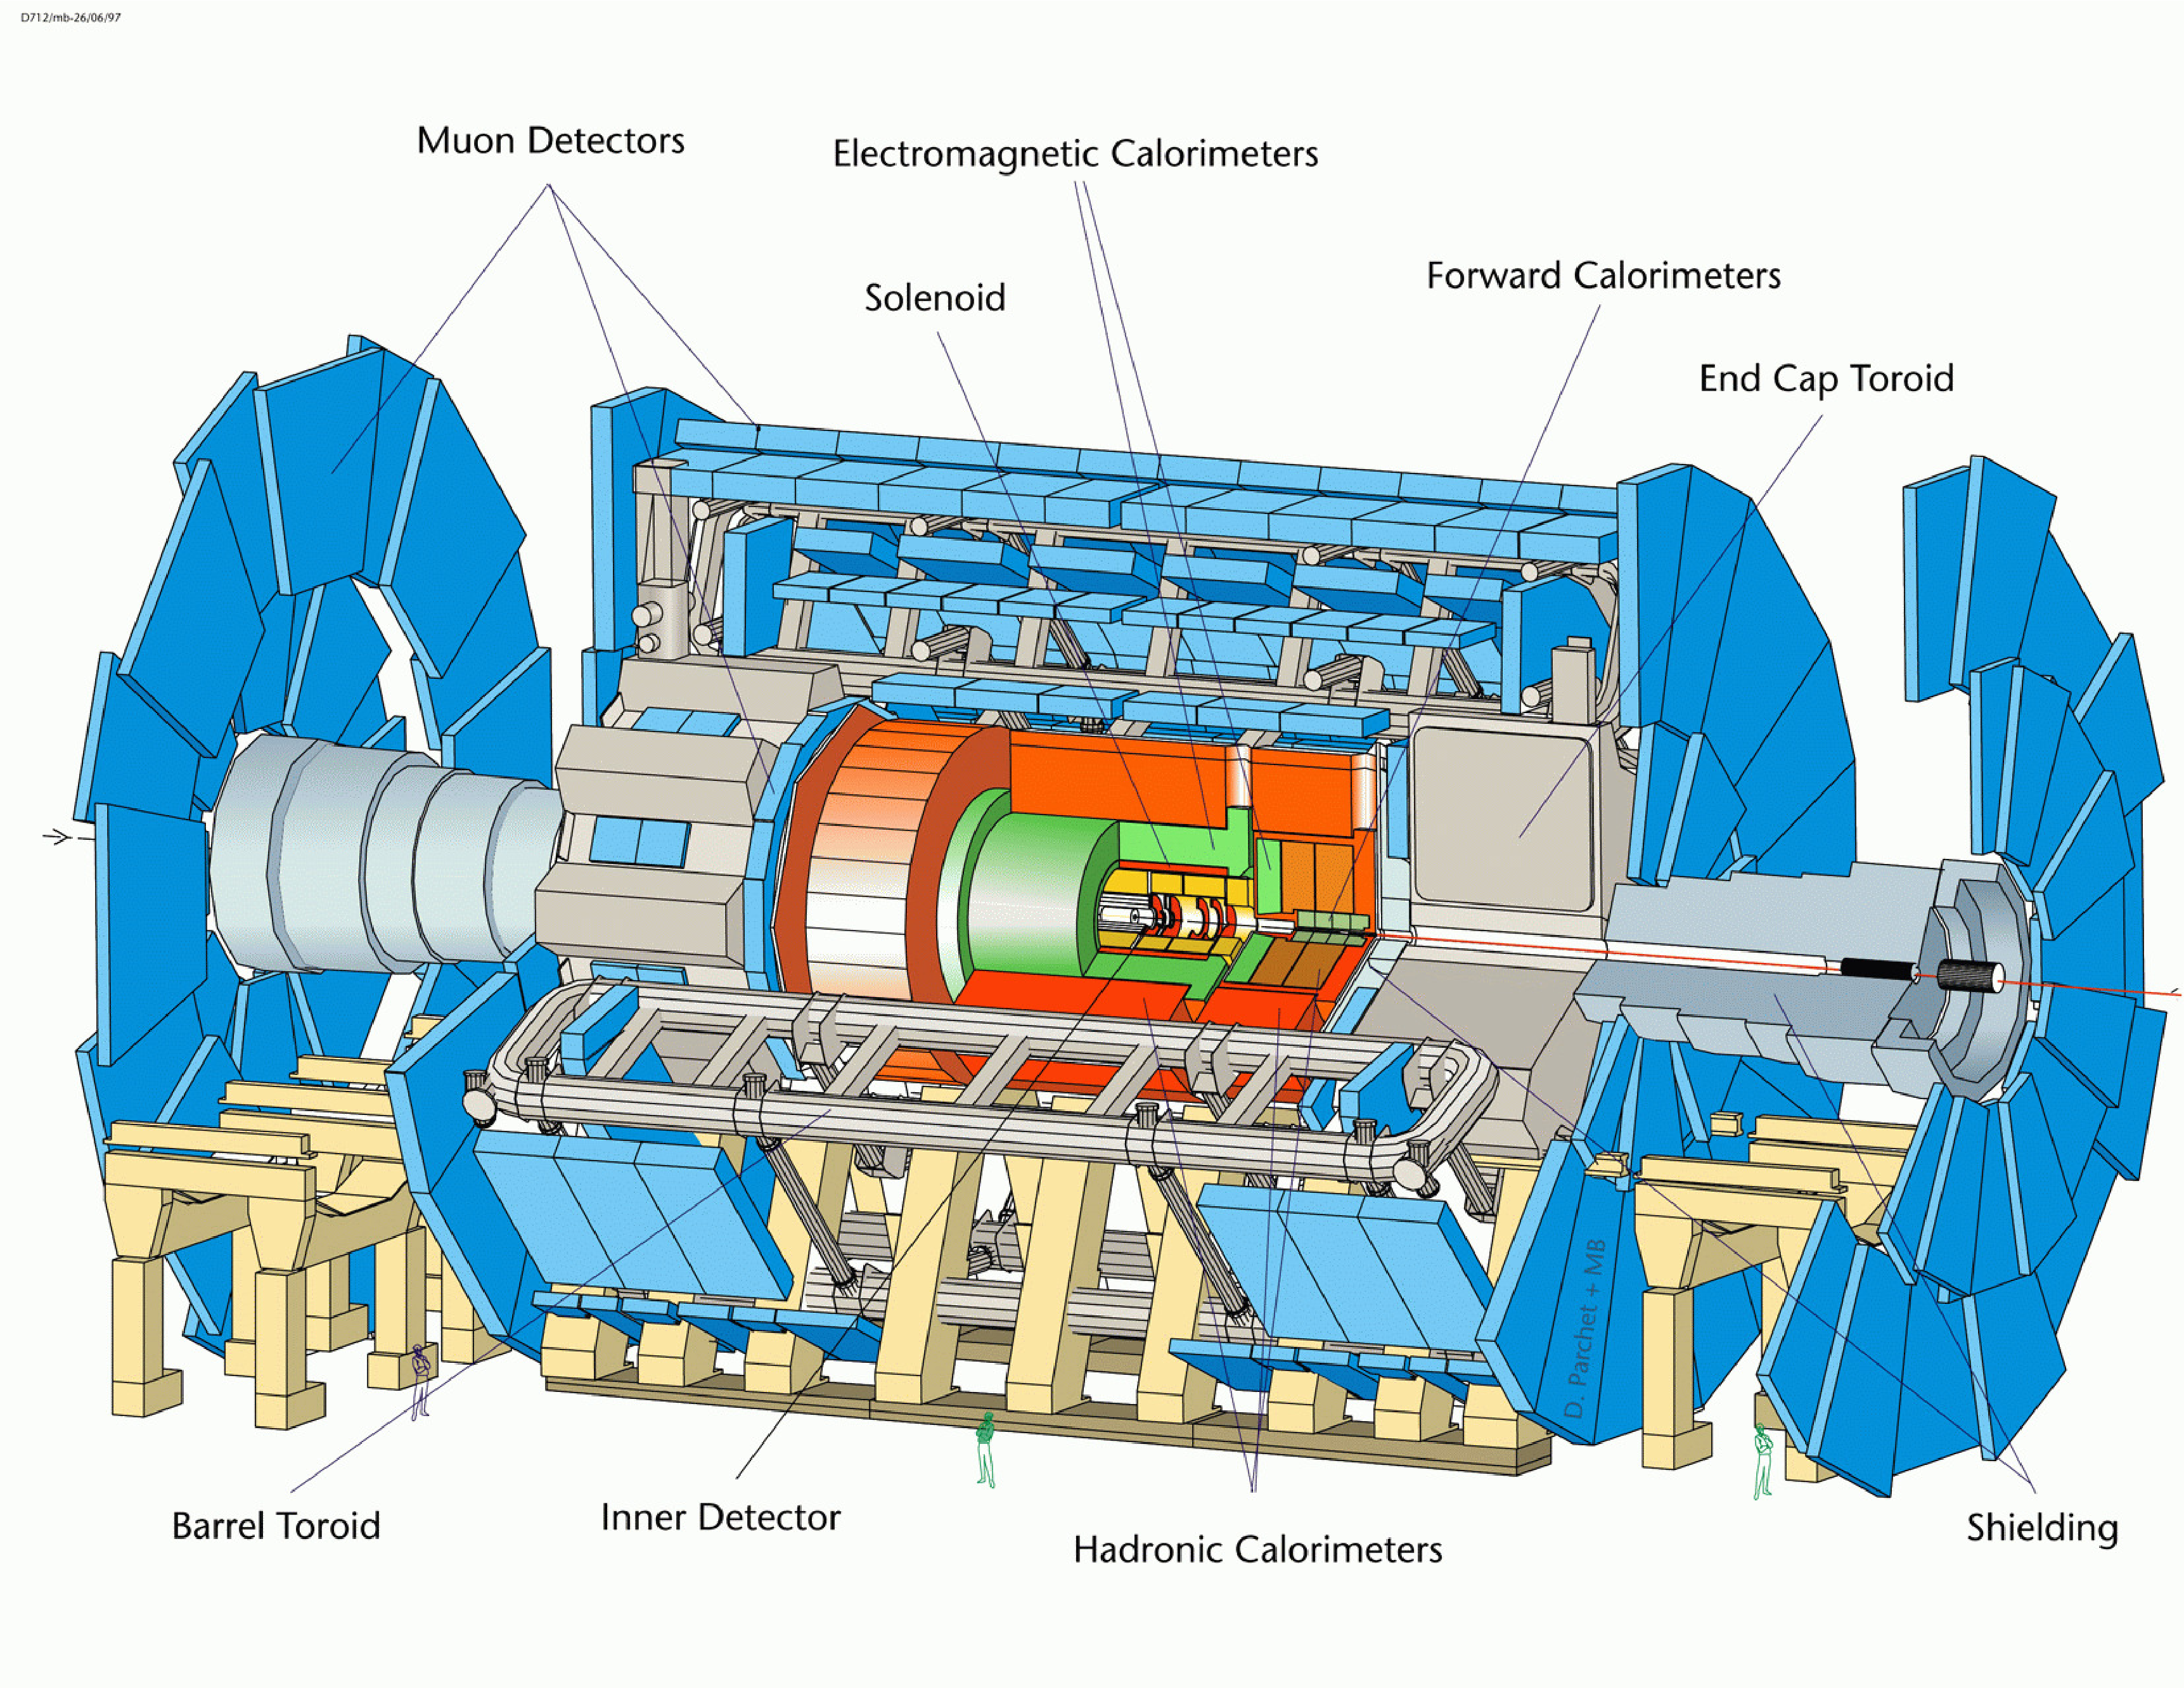
\includegraphics[angle=90,width=1\textwidth]{Fig2/TDRchapter1_fig1_ATLAS_DETECTOR.pdf}
    \caption{El detector de ATLAS}
    \label{fig:ATLAS}
  \end{center}
\end{figure}


%------------------------------------------------------------------------
\subsection{The Inner Detector}\label{sec:atlasID}
%------------------------------------------------------------------------
El detector interno de ATLAS (figura \ref{fig:figinner}) est\'a contenido en un cilindro de 7 m de longitud y 1,15 m de radio exterior. El mismo ha sido dise\~nado para la reconstrucci\'on de trazas de part\'iculas cargadas en un campo magn\'etico solenoidal de 2 Tesla, con un rango de pseudorapidez que se extiende hasta $|\eta|=  2.5$. Est\'a compuesto por tres subdetectores: el  detector de p\'ixeles , el detector de microbandas de silicio (SCT, del ingl\'es \emph{Semiconductor Tracker}) y el de transici\'on de radiaci\'on (TRT, \emph{Transition Radiation Tracker}).  La combinaci\'on de estas tecnolog\'ias permite el reconocimiento de trazas de manera robusta y una alta precisi\'on en las coordenadas $\eta$ y $\phi$.  

   Desde el punto de vista mec\'anico el detector consiste en un barril extendido en la coordenada \emph{z} sobre $\pm$ 80 cm, y dos ruedas o tapas laterales id\'enticas cubriendo el resto de la cavidad. En la regi\'on del barril todos los elementos de detecci\'on est\'an ordenados en estructuras cil\'indricas, mientras que en las tapas dichos elementos est\'an montados en discos perpendiculares a la direcci\'on del haz. Esto asegura que las part\'iculas pasen todos los elementos de detecci\'on con \'angulos de incidencia grandes.

\begin{figure}[htbp]
  \begin{center}
      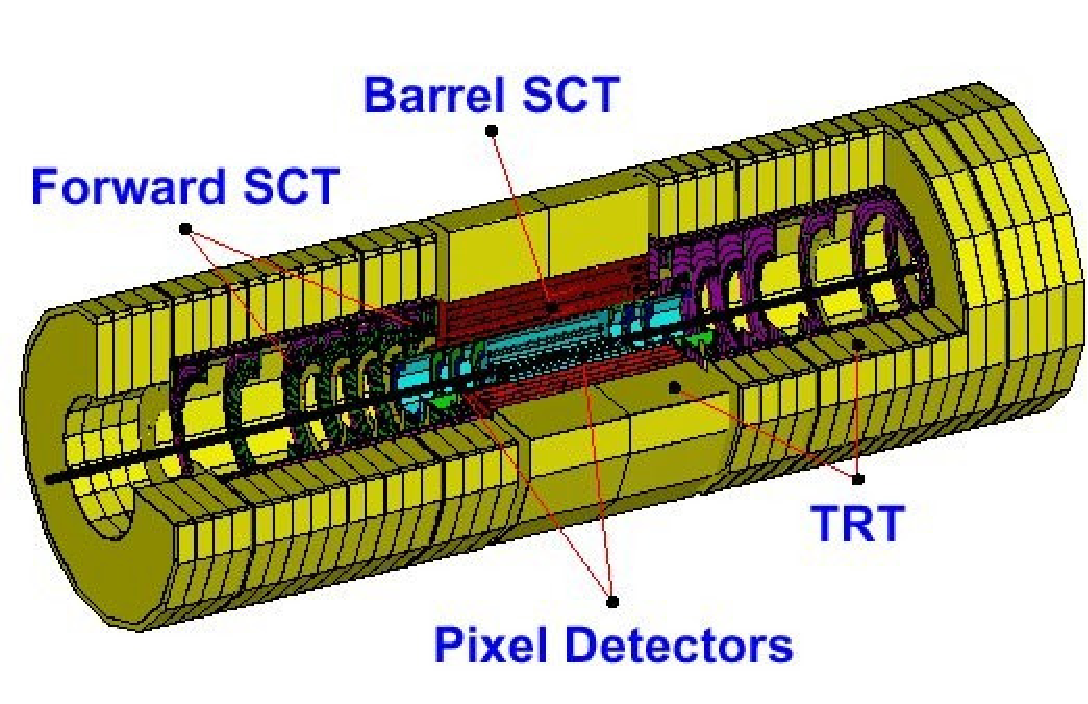
\includegraphics[width=0.9\textwidth]{Fig2/innnerdetector3d.pdf}
    \caption{Vista del detector interno de ATLAS. Se indican las posiciones del barril central y partes laterales del SCT, el detecor de p\'ixeles y el TRT}
    \label{fig:figinner}
  \end{center}
\end{figure}

%\subsubsection{Los detectores de  silicio}
%   El sistema de detectores de silicio est\'a dise\~nado  para proveer 11 mediciones de precisi\'on por traza en la regi\'on radial intermedia, contribuyendo a la medici\'on del momento, el par\'ametro de impacto y la posici\'on del v\'ertice.  Para ello dos tecnolog\'ias son implementadas: detectores de p\'ixel y detectores de microbandas de silicio. 

\subsubsection{El detector de p\'ixeles}

   Este sistema consiste en tres barriles de $\sim$ 4, 10 y 13 cent\'imetros de radio medio, respectivamente; y 5 discos a cada lado. Contiene 140 millones de elementos detectores de forma cuadradra,  cada uno de 50 $\mu$m en la direcci\'on R$\phi$ y 300 $\mu$m en z, midiendo as\'i dos coordenadas por cada m\'odulo detector. Todo el dispositivo est\'a situado tan cerca como es posible del punto de interacci\'on, entregando 3 mediciones de alta precisi\'on y granularidad en la regi\'on cercana al punto de interacci\'on primario, contribuyendo a la medici\'on del par\'ametro de impacto y la posici\'on del v\'ertice.

\subsubsection{El detector de microbandas de silicio}
% Ver esto

   El sistema de detecci\'on por microbandas de silicio consta de cuatro cilindros conc\'entricos; de 300, 373, 447 y 520 mm de radio, respectivamente, compuestos, cada uno de ellos, por  m\'odulos detectores montados en estructuras de fibra de carb\'on. Cada m\'odulo posee dos capas de microbandas. En la primera, las bandas est\'an dispuestas paralelas al eje del haz midiendo as\'i la cordenada $\phi$ directamente. \'Estas, junto con las microbandas en la capa siguiente, con un \'angulo \emph{stereo} de 40 mrad, reconstruyen la coordenada \emph{z}. A los lados del barril central se tienen dos tapas con m\'odulos montados en 9 ruedas. La resoluci\'on espacial en el sistema es de 16 $\mu$m en R$\phi$ y 580 $\mu$m en \emph{z}.

   %El sistema de detecci\'on por bandas de silicio consiste en 8 capas de dichas microbandas, dispuestas en m\'odulos, teniendo dos capas por cada m\'odulo detector. Estos  m\'odulos est\'an montados en estructuras cil\'indricas de fibra de carb\'on dando lugar a cuatro barriles de 300, 373, 447 y 520 mm de radio, respectivamente. En una de las capas del detector las bandas est\'an dispuestas paralelas al eje del haz midiendo as\'i la cordenada $\phi$ directamente. Esta capa, junto con las bandas en la capa posterior, con un \'angulo \emph{stereo} de 40 mrad, reconstruyen la coordenada \emph{z}. En las tapas, los m\'odulos detectores est\'an montados en anillos sobre nueve ruedas, que se encuentran tambi\'en unidas mediante un marco que las contiene.  La resoluci\'on espacial en el sistema de bandas es de 16 $\mu$m en R$\phi$ y 580 $\mu$m en \emph{z}. 

  Tendremos, t'ipicamente, 8 capas de bandas de silicio (m\'as las tres de p\'ixeles) atravesadas por cada traza proveniente del punto de interacci\'on. Un impacto (o \emph{hit}) en una de las capas se referir\'a a un canal de detecci\'on con una se\~nal de salida sobre un determinado umbral de energ\'ia. En el caso del detector de silicio, tendremos un cluster peque\~no de canales, creado por una part\'icula cargada o ruido. Dos impactos correspondientes a una misma traza, en las dos capas de un m\'odulo detector contribuyen a un punto tridimensional en el espacio que llamaremos SP, del ingl\'es \emph{Space Point}. 


\subsubsection{El detector de radiaci\'on de transici\'on}

   %ESTO ES MENOR
   %El detector de radiaci\'on de transici\'on se basa en el hecho de que cuando una part\'icula cargada atraviesa materiales con distinta constante diel\'ectrica emite radiaci\'on que depende del cociente energ\'ia a masa, permitiendo as\'i la identificaci\'on de las part\'iculas.
% el uso de hilos met\'alicos aislados contenidos en vol\'umens individuales de gas
 
  El detector de radiaci\'on de transici\'on de ATLAS est\'a basado en el uso de tubos detectores del di\'ametro de una pajita de gaseosa, para la identificaci\'on y reconstrucci\'on de las trayectorias de part\'iculas cargadas. En total hay alrededor de 370000 tubos de 4 mm de di\'ametro y 144 de longitud en todo el detector, y, en virtud de su peque\~no di\'ametro pueden operar a las altas frecuencias esperadas en el LHC. % llenados con una mezcla  gaseosa (70 $\%$ xen\'on), para la absorci\'on de la radiaci\'on de transici\'on.
   
  Cada tubo contiene en su interior un hilo de tungsteno, cubierto de oro, de 30 $\mu$m de di\'ametro y est\'a relleno de una mezcla gaseosa (70 $\%$ xen\'on) que se ioniza cuando pasa una part\'icula. La medici\'on del tiempo de arribo de los iones producidos al hilo central, permite determinar la posici\'on del impacto dentro del radio del tubo. %atravesado por dicha part\'icula. 
  Los tubos detectores est\'an orientados de manera radial (en ruedas) en las tapas y, a lo largo del eje del haz , en la regi\'on del barril. Estas orientaciones han sido elegidas para maximizar el n\'umero de tubos atravesados en todas las direcciones.  La secci\'on del barril consiste en m\'odulos individuales de entre 329 y 793 tubos axiales, cubriendo el rango radial de 56 a 107 cm.  

   La detecci\'on de radiaci\'on de transici\'on, provocada por la existencia de materiales de distinto \'indice de refracci\'on entre los tubos, generar\'a se\~nales m\'as intensas y permitir\'a una mejor identificaci\'on de electrones que atraviesan el detector (los muones tambi\'en emiten radiaci\'on de transici\'on pero al ser mucho m\'as masivos que los electrones, lo hacen en una cantidad mucho menor).

   Este sistema de detecci\'on por tubos provee un gran n\'umero de puntos por traza (t\'ipicamente 36 puntos), lo cual determina un seguimiento cont\'inuo de la misma, con mucho menos material por punto y menor costo (mucho menor comparado con la tecnolog\'ia de p\'ixeles implementada en el subdetector m\'as interno).  La gran cantidad de puntos o impactos por traza es un instrumento poderoso en la b\'usqueda y reconstrucci\'on de trazas en el detector interno.

%------------------------------------------------------------------------
\subsection{The Calorimeters}\label{sec:atlasCALO}
%------------------------------------------------------------------------
 El sistema de imanes superconductores de ATLAS consiste en un solenoide central que provee el campo magn\'etico necesario al detector interno, rodeado por un arreglo de bobinas o bucles, con forma de pista de carrera, que generan un campo magn\'etico toroidal para el espectr\'ometro de muones.Todo el sistema es enfriado de manera indirecta mediante el flujo de helio l\'iquido a 4,5 K.

   El solenoide es un electroim\'an superconductor de 5,3 m de largo, situado en el interior del calor\'imetro electromagn\'etico. Comparte el cri\'ostato con el calor\'imetro de arg\'on l\'iquido, evitando la presencia de dos paredes criost\'aticas y reduciendo as\'i la cantidad de material introducido. La longitud del solenoide es considerablemente m\'as peque\~na que la del barril del detector de trazas. Este es el resultado de un compromiso: un bobinado corto reduce la cantidad de material introducido mientras que uno largo proporciona un campo magn\'etico m\'as uniforme en dicho detector. El campo magn\'etico a lo largo del eje \emph{z} es de 2 T en el punto de interacci\'on.
% existe .criost\'aticas.?

   El arreglo de bobinas est\'a dividido en un barril central y dos regiones laterales, al igual que los detectores. El barril central est\'a constituido por 8 bobinas de 5 m de ancho por 25 metros de largo aproximadamente, dispuestas sim\'etricamente alrededor del haz de manera radial. Las bobinas del barril se encuentran en cri\'ostatos separdos, mientras que las 8 bobinas en cada una de las tapas o toroides laterales est\'an ubicadas en un cri\'ostato com\'un.

   Con un campo magn\'etico toroidal las part\'iculas atravesar\'an todo el rango de pseudorapidez casi perpendicularmente al haz. El n\'umero peque\~no de bobinas que generan el campo toroidal resulta en una intensidad de campo que var\'ia fuertemente con la coordenada $\phi$. En el barril el campo magn\'etico es de 2 T, mientras que en las tapas es de 4 T en las zonas de mayor intensidad.   
    
\subsubsection{El calor\'imetro}

   Una vez que la part\'icula atraviesa el detector interno, ingresa al calor\'imetro. Un detector calorim\'etrico est\'a dise\~nado para absorber la energ\'ia de las part\'iculas que lo atraviesan y se encuentra dividido normalmente en un calor\'imetro electromagn\'etico y uno hadr\'onico dado el diferente comportamiento de fotones/electrones por un lado, y hadrones por el otro.  As\'i el calor\'imetro de ATLAS consiste en un sector electromagn\'etico que cubre una regi\'on de pseudorapidez $|\eta|<3.2$ (barril y tapas),  y uno hadr\'onico formado por tres partes: un gran barril cubriendo la zona de $|\eta|<1.7$, dos tapas en los extremos cubriendo la regi\'on de $1.5<|\eta|<3.2$, y calor\'imetros de bajo \'angulo cubriendo la regi\'on de pseudorapidez de  $3.1 <|\eta|< 4.9$. % Para la identificaci\'on de energ\'ia transversa faltante el calor\'imetro debe constar de una alta hemeticidad lo que significa que la cobertura en pseudorapidez debe alcanzar $|\eta|<5$. 

\subsubsection{El calor\'imetro de arg\'on l\'iquido}
  
   El calor\'imetro electromagn\'etico de ATLAS consiste en un gran barril interno y dos ruedas (\emph{end-caps}), una a cada lado del mismo. Se trata de un calor\'imetro de muestreo que funciona con arg\'on l\'iquido (se denomina de muestreo porque mide s\'olo una fracci\'on de la energ\'ia depositada por la part\'icula incidente). Est\'a formado por placas de plomo/acero inoxidable intercaladas con electrodos de cobre; el espacio entre ambos se llena con arg\'on l\'iquido, permitiendo la deriva de los electrones de ionizaci\'on bajo el alto voltaje aplicado. 

  Con el fin de asegurar una perfecta cobertura en todo el rango de pseudorapidez  y proveer una completa simetr\'ia en la coordenada $\phi$ se ha elegido una geometr\'ia en forma de acorde\'on. En la regi\'on dedicada a f\'isica de precisi\'on ($|\eta|<2.5$) el calor\'imetro electromagn\'etico est\'a dividido en cuatro secciones de muestreo. La primera o \emph{Presampler} consiste en una delgada capa de arg\'on desprovista de material absorbente, cuyo prop\'osito es la correcci\'on por la p\'erdida de energ\'ia  en el solenoide y las paredes del cri\'ostato. La segunda secci\'on posee una profundidad de 4.3$X_{0}$\footnote{$X_{0}$ es el s\'imbolo utilizado para la Longitud de Radiaci\'on (\emph{Radiation length}), definida como la distancia media sobre la cual un elect\'on muy energ\'etico pierde $1/e$ de su energ\'ia por bremsstrahlung o bien, como $7/9$ del camino libre medio en la producci\'on de pares. Contituye una escala de longitud apropiada para describir cascadas electromagn\'eticas de alta energ\'ia.} y en ella la lectura se lleva a cabo mediante celdas en forma de tiras delgadas en $\eta$, dando una buena resoluci\'on en dicha coordenada, con $\Delta\eta=0.0031$. La secci\'on de \emph{2nd Sampling} (16$X_{0}$) es donde se deposita la mayor\'ia de la energ\'ia, teniendo ambas coordenadas igual importancia. All\'i el tama\~no de celda es de $\Delta\phi\Delta\eta=0.0245\times 0.0245$. S\'olo los electrones m\'as energ\'eticos llegar\'an a la cuarta secci\'on de muestreo (\emph{3rd Sampling}).

   Las ruedas calorim\'etricas comienzan en $|\eta|=1.5$ y contin\'uan abajo hasta $|\eta|=3.2$, pero con un tama\~no de celda mayor por encima de $|\eta|=2.5$.

   En la regi\'on de bajo \'angulo, el calor\'imetro hadr\'onico funciona tambi\'en con arg\'on l\'iquido de manera de resistir los altos niveles de radiaci\'on. Su dise\~no es m\'as sencillo que el del calor\'imetro electromagn\'etico y como absorbentes posee placas paralelas de cobre, perpendiculares al haz. La regi\'on de esta parte del calor\'imetro hadr\'onico, que cubre hasta $|\eta|=4.9$, est\'a hecha de cobre/tungsteno. La elecci\'on de este material es necesaria para limitar el ancho y la profundidad de las lluvias provenientes de jets de altas energ\'ias cercanas a la l\'inea del haz. %and to sep the background levels low in the surrounding calorimeteres from particles spraying out from the forward region.

\subsubsection{El calor\'imetro hadr\'onico de tejas}
% TileCal [ ] Tile Calorimeter Technical Design Report, CERN/LHCC 96-42, 15-12-1996;

   El calor\'imetro hadr\'onico de tejas de ATLAS est\'a compuesto por tres barriles, uno central de 5,6m y dos extensiones de 2,9m cada una. El radio interno es de 2,2m y el externo, de 4,2m.  

   Cada barril est\'a dividido en 64 cu\~nas azimutales o m\'odulos, con una estructura peri\'odica en la direcci\'on paralela al haz. Cada m\'odulo es una estructura de tejas de hierro (material absorbente) alternadas con tejas de pl\'astico centellador, dispuestas en un plano paralelo al eje del haz.  Los materiales centelladores emiten luz en forma de peque\~nos pulsos cuando son atravesados por part\'iculas o radiaci\'on; acoplando el centellador a un fotomultiplicador el pulso de luz se convierte en un pulso el\'ectrico que puede ser analizado.  En el caso del calor\'imetro hadr\'onico de ATLAS, cuando una part\'icula atraviesa una teja centelladora emite luz en el rango del ultravioleta, de intensidad proporcional a la energ\'ia depositada por la part\'icula. 

   Se ha elegido una segmentaci\'on proyectiva en torres de $\Delta\phi\Delta\eta=0.1\times 0.1$ y cada una de estas torres est\'a dividida, en profundidad, en tres celdas, le\'idas individualmente por dos fotomultiplicadores para conseguir redundancia en la se\~nal. La luz generada en las tejas es recogida mediante fibras \'opticas que cambian la longitud de onda y transportada a los fotomultiplicadores (este subdetector posee unos 10.000 fotomultiplicadores).

   El calor\'imetro hadr\'onico debe tener el espesor suficiente para contener la energ\'ia de los hadrones. Con este prop\'osito y para obtener una buena resoluci\'on se han elegido 11 longitudes de absorci\'on como camino previo a las c\'amaras de muones.
 

%------------------------------------------------------------------------
\subsection{The Muon System}\label{sec:atlasCALO}
%------------------------------------------------------------------------
 El sistema de muones sirve a un doble prop\'osito: funciona como sistema de disparo (o \emph{trigger}) para la selecci\'on de eventos con muones de alta energ\'ia, y como espectr\'ometro de muones de alta precisi\'on. En este sentido, este detector llevar\'a a cabo la identificaci\'on de los muones producidos en las colisiones \emph{p-p}, determinando sus trayectorias y momentos.
% Las part\'iculas provenientes del punto de interacci\'on atraviesan tres conjuntos de c\'amaras, uno situado previo al toroide, uno interior y otro posterior. 
   El sistema consiste en un conjunto de toroides (llamamos as\'i, por su forma, a los tres conjuntos de bobinas que proveen el campo magn\'etico toroidal) y c\'amaras de tubos de deriva que se encuentran rodeando al calor\'imetro. En la parte del barril del detector, las c\'amaras est\'an situadas en el interior del toroide lo que permite la medici\'on del momento de las part\'iculas a partir de la desviaci\'on de sus trayectorias en el campo magn\'etico. En las tapas, donde la presencia del cri\'ostato impide posicionar las c\'amaras dentro del campo magn\'etico, el momento es medido a partir de la diferencia entre los \'angulos de entrada y salida del im\'an.
En el plano trasversal, tanto en la regi\'on del barril como en las tapas laterales, el sistema de c\'amaras estar\'a dividido en 16 sectores, siguiendo la simetr\'ia determinada por las 8 bobinas del barril central del sistema magn\'etico. Las c\'amaras cubren el espacio entre las bobinas, y todo el rango acimutal en la regi\'on que las rodea. Los sectores se numeran comenzando a partir de $\phi = 0$, en el sentido contrario de las agujas del reloj, teniendo en la direcci\'on vertical a los sectores 6 (en la parte superior del detector) y 13 (sector inferior).  

   Los c\'amaras de tubos de deriva (MDTs) son c\'amaras proporcionales hechas de tubos de aluminio de 30 mm de di\'ametro y longitudes variables de 70 a 630 cm, con un hilo central de 50$\mu$m de di\'ametro, de W-Re. En la regi\'on del barril dichas c\'amaras est\'an distribuidas en 3 capas cil\'indricas conc\'entricas (estaciones) alrededor del haz, de 5; 7,5 y 10 metros de radio. Los tubos est\'an dispuestos de manera transversal al eje \emph{z} de manera de medir la coordenada en el plano de desviaci\'on de la trayectoria de la part\'icula (plano \emph{Rz}).  Estas c\'amaras miden el tiempo de deriva de la ionizaci\'on producida por el paso del mu\'on, teniendo una resoluci\'on de 80 $\mu$m.
% MAS del TDR? Falta los radios de las estaciones(?)
   
   Cada c\'amara MDT est\'a cubierta por una o dos c\'amaras de placas resistivas (RPCs). Cada una de ellas encierra un volumen de gas entre planchas resistivas de baquelita, dotada una de ellas con tiras de electrodos. Dado que los tubos de deriva poseen un di\'ametro relativamente grande que resulta en un tiempo de deriva m\'aximo de 480ns, mucho mayor que los 25 ns entre cruce de \emph{bunches}, se requieren c\'amaras especiales de disparo para la selecci\'on de eventos. La funci\'on de trigger en el barril es provista por tres capas de RPCs, situadas, dos de ellas, a ambos lados de la segunda estaci\'on de MDTs y la restante, en la cara interior de la estaci\'on m\'as externa. 
En las tapas, esta funci\'on es cumplida por tres estaciones de TGCs (\emph{Thing Gap Chambers}). Estas c\'amaras son similares en dise\~no a c\'amaras prporcionales multihilo, con la diferencia de que poseen una distancia c\'atodo-c\'atodo menor que la pendiente del \'anodo (hilo). 
   Las c\'amaras de disparo proveen una estimaci\'on de las coordenadas $\phi$ y $\eta$ del punto de impacto de la traza, mientras que las c\'amaras MDTs dar\'an (con mayor precisi\'on) la coordenada $\eta$.

    En la regi\'on de bajo \'angulo, donde la densidad de trazas es mayor, se utilizan c\'amaras de tiras de c\'atodos (CSCs) de granularidad m\'as fina comparadas con las MDTs, para la detecci\'on de trayectorias. Estas c\'amaras son c\'amaras proporcionales, con un espacio entre hilo de 2,5 mm. Cada una de ellas proporciona medida de dos coordenadas y puede operar en condiciones de alto campo magn\'etico.

   En la figura \ref{fig:MUON1} se puede ver un esquema del espectr\'ometro de muones, donde se indica la posici \'on de las diferentes c\'amaras descriptas.

\begin{figure}[htbp]
  \begin{center}
      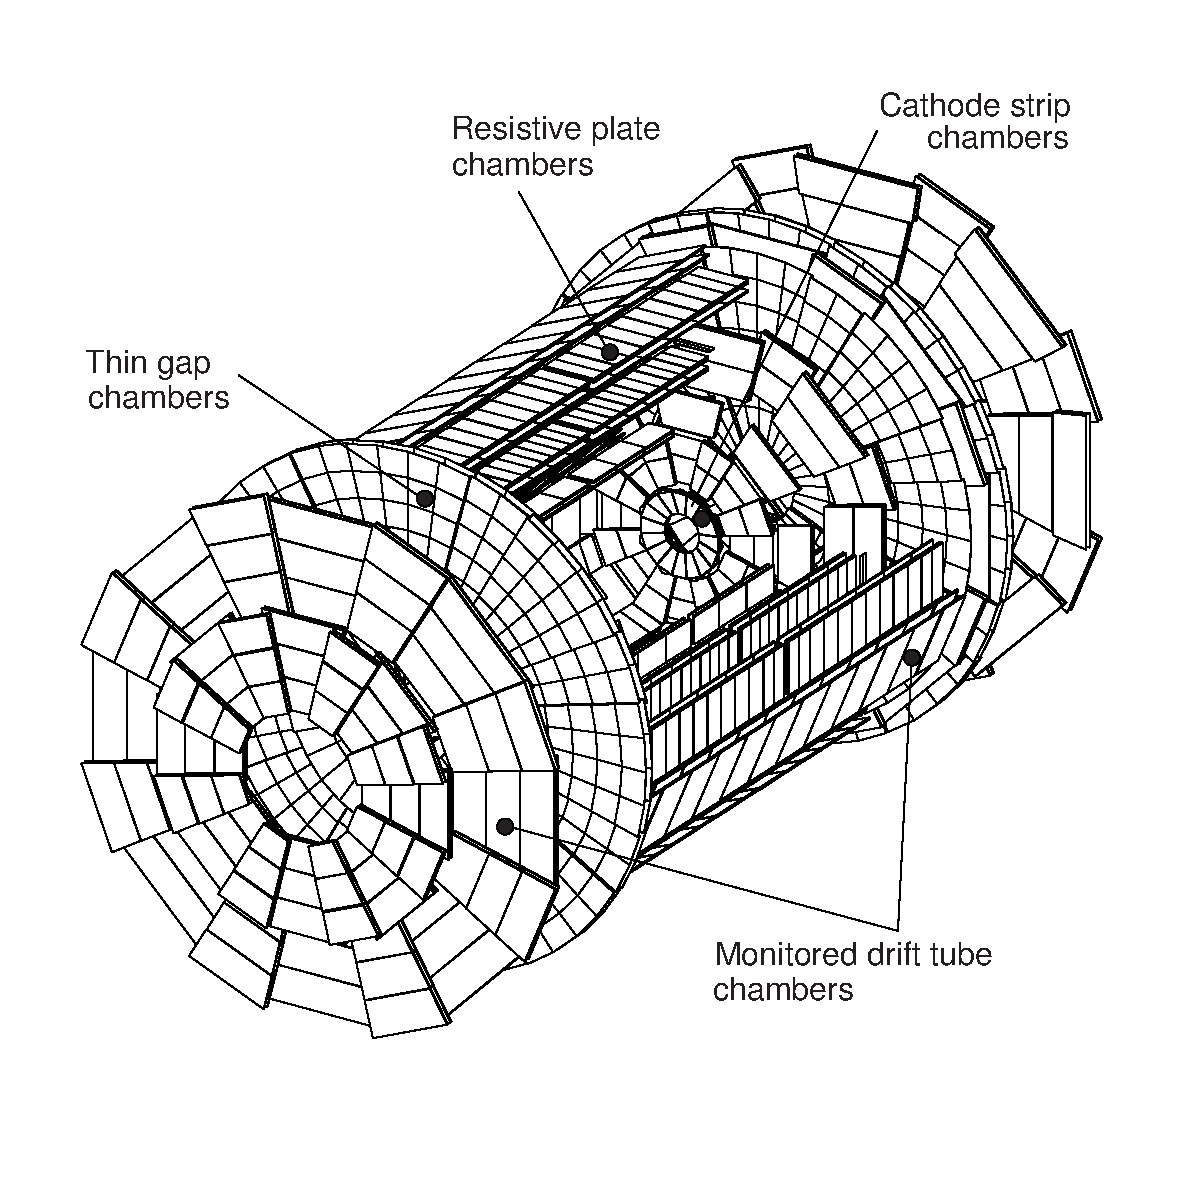
\includegraphics[width=0.8\textwidth]{Fig2/muonspectrometeradele-bw.pdf}
    \caption{Vista tridimensional del espectr\'ometro de muones de ATLAS, indicando las \'areas cubiertas por las diferentes c\'amaras que lo componen}
    \label{fig:MUON1}
  \end{center}
\end{figure}



%------------------------------------------------------------------------
\subsection{Trigger and Data Adquisition}\label{sec:atlasCALO}
%------------------------------------------------------------------------
 En este cap\'itulo se analiza la estructura del trigger de ATLAS, y el sistema de adquisici\'on y flujo de los datos. Se presenta, asimismo, una breve descripci\'on de los algoritmos usados en la reconstrucci\'on de trayectorias para la selecci\'on de eventos en el detector interno. 


\subsubsection{Arquitectura general}

   El sistema de Trigger y Adquisici\'on de Datos\cite{TDRtdaq} de ATLAS est\'a basado en tres niveles de selecci\'on \emph{online}: Nivel 1, Nivel 2 y Filtro de Eventos. Cada nivel es m\'as lento pero m\'as preciso que el anterior. Trabajando con una frecuencia de interacci\'on de $10^{9}$ Hz y luminosidades del orden de $10^{34}$ $cm^{-2}$ $s^{-1}$, este sistema ser\'a el encargado de reducir la frecuencia de eventos inicial de 40 MHz a 200Hz, que es la velocidad con la que pueden almacenarse. 

   En la figura \ref{fig:TDAQ} se muestra un vista simplificada de los principales componentes y funciones.  

\begin{figure}[!h]
\begin{center}
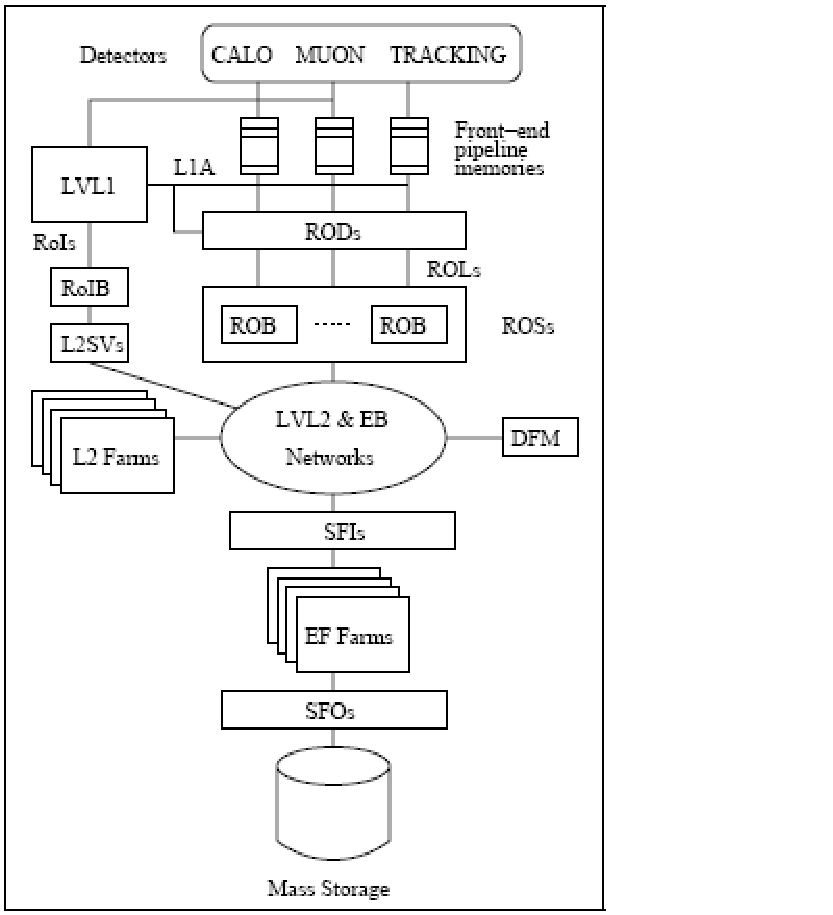
\includegraphics[width=0.5\textwidth]{Fig3/paint_TDAQ.pdf}
\caption{Principales componentes del sistema de trigger y adquisici\'on de datos de ATLAS. } 
\label{fig:TDAQ}
\end{center}
\end{figure}

   El mecanismo que lleva a cabo el movimiento de la informaci\'on (Data Flow System), es el responsable de recibir los datos de los detectores, pasando parte de ellos al sistema de trigger y enviando luego, los eventos seleccionados al lugar de almacenamiento. Siguiendo el esquema de la figura, la comunicaci\'on entre los \emph{drivers} de lectura %controladores de lectura?
de cada detector (RODs) y el sistema de adquisici\'on de datos, est\'a dada por los \emph{buffers} de almacenamiento transitorio (ROBs). La informaci\'on de los eventos aceptados por el Nivel 1 son transportados de los primeros al sistema de lectura (ROS), que consta de numerosos ROBs, guardando los datos a la espera de la decisi\'on del trigger. La informaci\'on requerida por el segundo nivel es provista por estos \'ultimos. Los eventos aceptados son reconstruidos (a partir de fragmentos contenidos en diferentes ROBs) y pasados al siguiente nivel.
%(\emph{Read Out Drivers})
%(\emph{Read Out Buffers})
% (\emph{Read Out System})

   El Nivel 2 y el Filtro de Eventos componen el \emph{High-level Trigger} (HLT) de ATLAS. El Nivel 2 trabaja a la frecuencia de aceptaci\'on del Nivel 1, utilizando una secuencia de r\'apidos algoritmos de selecci\'on que operan t\'ipicamente sobre una fracci\'on de los datos del evento, contenida en regiones del detector previamente seleccionadas por ese nivel (ver el mecanismo de la regi\'on de inter\'es en la siguiente secci\'on). Si la decisi\'on del Nivel 2 es rechazar el evento, los datos del mismo son eliminados de los buffers correspondientes. Si el evento es aceptado,  se reconstruye  en el EB (Event Builder) y es pasado al Filtro de Eventos. Este nivel ejecutar\'a algoritmos de reconstrucci\'on m\'as sofisticados, adaptados de aquellos para el an\'alisis \emph{offline}, utilizando informaci\'on detallada de los detectores para efectuar el proceso de selecci\'on final, que determinar\'a cu\'ales son los eventos que ser\'an guardados para posteriores estudios.

  En las siguientes secciones se presenta una descripci\'on m\'as detallada de los niveles de trigger.

 
\subsubsection{El Nivel 1}

   El primer nivel de trigger de ATLAS es implementado mediante hardware. \'Este realiza una decisi\'on inicial a partir de la informaci\'on provista por los calor\'imetros y del detector de muones, basando su estrategia en la combinaci\'on de objetos en coincidencia. %or veto.
  
   En el sistema de muones, los candidatos de alto momento transverso son identificados en las c\'amaras especiales de trigger: RPCs en el barril y TGCs en las tapas. En el caso del calor\'imetro, se definen una serie de conjuntos de umbrales de $p_T$ para cada objeto (electrones, fotones, jets, etc.), seleccionando aquellos que pasen los criterios de selecci\'on correspondientes al evento f\'isico de inter\'es. 

   Puesto que la decisi\'on de aceptar un evento no puede ser realizada en los 25 ns que median entre dos cruces de \emph{bunches}, los subdetectores almacenan localmente la informaci\'on del mismo en \emph{pipelined buffers} hasta que el Nivel 1 efect\'ua la selecci\'on. Luego, los datos son enviados a los RODs especi\'ficos de cada detector para luego dirigirse a los ROBs, donde son almacenados hasta que la decisi\'on del Nivel 2 sea alcanzada. 
   Cuando un evento es aceptado, el Nivel 1 comunica la decisi\'on al mecanismo que se encargar\'a de construir una Regi\'on de Inter\'es (RoI). Este mecanismo es una importante pieza sobre la que descansa la estrategia del sistema de trigger; a trav\'es del mismo, el Nivel 2 har\'a uso de la informaci\'on del evento en regiones localizadas del detector, de manera que los algoritmos de reconstrucci\'on en ese nivel s\'olo transfieran los ROBs necesarios para arribar a una r\'apida decisi\'on. %Es importante notar que la informaci\'on de todos los subdetectores est\'a disponible para dichos algoritmos en caso de ser necesario.
La RoI contendr\'a la informaci\'on de la posici\'on ($\eta$ y $\phi$) y el momento de los objetos candidatos.

   Este nivel est\'a dise\~nado para llevar a cabo su decisi\'on en un tiempo menor a 2.5 $\mu$s, medidos desde la colisi\'on \emph{p-p}, hasta que la informaci\'on del evento est\'a disponible en la electr\'onica de salida de los detectores. En este proceso la frecuencia de eventos ser\'a reducida a 75KHz (l\'imite fijado por la electr\'onica).

\subsection{El HLT}

 El High-level Trigger de ATLAS abarca la segunda y tercera etapa de la selecci\'on de eventos. Comprende el Nivel 2 y el Filtro de Eventos, y contiene adem\'as, el Software de Selecci\'on (ESS). Este \'ultimo comparte la estructura usada por el Offline para los c\'odigos de selecci\'on, facilitando el an\'alisis \emph{offline} de los datos, y el desarrollo de algoritmos en el HLT.

   El punto de entrada del trigger es el resultado del Nivel 1. \'Este provee informaci\'on acerca de la regi\'on de inter\'es, fundamental para el r\'apido funcionamiento de los algoritmos del Nivel 2. As\'i, los datos del Nivel 1 gu\'ian la selecci\'on del Nivel 2; y \'esta a su vez guiar\'a la del Filtro de eventos, como se ilustra en la figura \ref{fig:HLTchainseed}. 
%HLTchain_seeding.pdf
\begin{figure}[!h]
\begin{center}
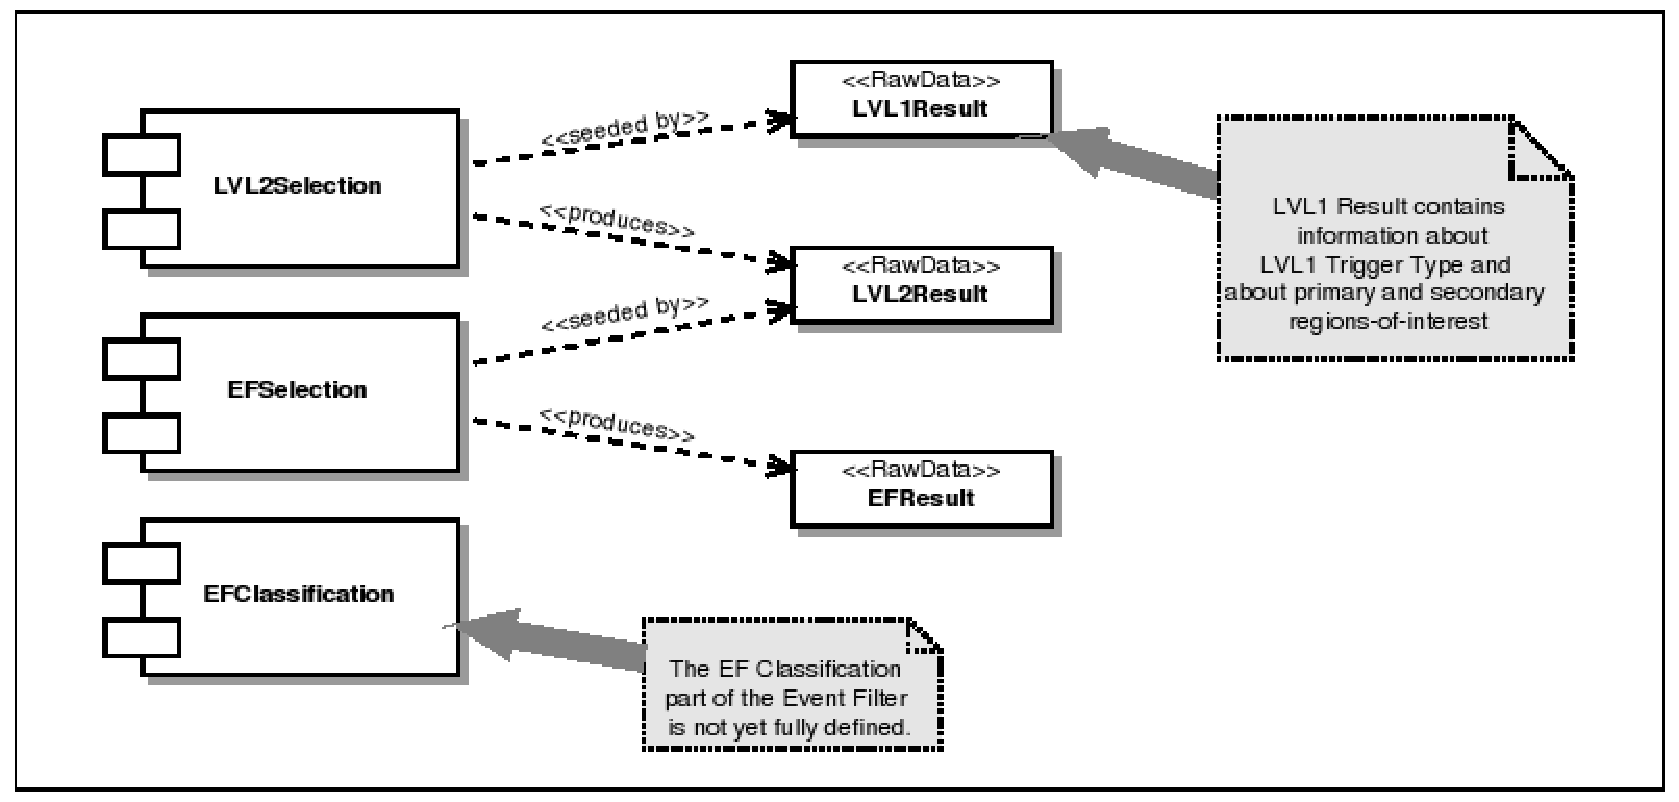
\includegraphics[width=0.9\textwidth]{Fig3/HLTchain_seeding.pdf} 
\caption{Cadena de selecci\'on del \emph{High-level Trigger} de ATLAS. Cada nivel es guiado por el resultado del paso anterior.}
\label{fig:HLTchainseed}
\end{center}
\end{figure}


\subsubsection{El Nivel 2}
   La tarea espec\'ifica del Nivel 2 es reducir la frecuencia de eventos de $\sim$ 100 kHz a alrededor de 2 kHz, combinando la informaci\'on de todos los detectores para su decisi\'on global. A diferencia del Nivel 1, esta segunda etapa de selecci\'on realiza operaciones no sincronizadas sobre los eventos, con un tiempo de decisi\'on de 10 ms.
%asynchronous??

   El Nivel 2 utiliza las regiones de inter\'es provistas por el Nivel 1. Cada regi\'on es examinada en el subdetector de origen (calor\'imetro o sistema de muones) para su confirmaci\'on; para luego buscar informaci\'on de otros subdetectores. En el caso del trigger de muones, el poder de rechazo del Nivel 2 proviene de ajustar los umbrales de $p_{T}$, respecto de los utilizados en el primer nivel, a partir de la informaci\'on de las c\'amaras de precisi\'on del sistema de muones (MDTs) y la correspondiente al detector interno.
Los procesadores del Nivel 2 son los encargados de ejecutar luego el software de selecci\'on de eventos, utilizando la informaci\'on almacenada en los \emph{buffers}. Usando las RoIs del Nivel 1, el Nivel 2 acceder\'a de manera selectiva a los datos en los ROBs, moviendo s\'olo la informaci\'on requerida para efectuar la decisi\'on. T\'ipicamente, s\'olo una peque\~na fracci\'on del detector, correspondiente a las regiones centradas en los objetos indicados por el Nivel 1, ser\'an necesitados por el segundo nivel.

  Hasta que un evento es aceptado o rechazado (en $\sim$ 10 ms), los datos son retenidos en los ROBs. En caso de aceptaci\'on, los fragmentos del evento almacenados en distintos buffers ser\'an requeridos por el sistema de control del Nivel 2 (L2SVs) para ser enviados al constructor de eventos (EB). El evento ensamblado es guardado en una \'unica direcci\'on de memoria para ser utilizado por el Filtro de Eventos. El tama\~no promedio de un evento ser\'a del orden de 1,5 MB.


\subsubsection{El Filtro de Eventos}

  Luego del Nivel 2, la \'ultima etapa de selecci\'on \emph{online} es realizada por el Filtro de Eventos (EF). El EF emplea algoritmos y m\'etodos similares a los implementados en el an\'alisis \emph{offline}, adaptados para su corrida en el tiempo real del experimento; su poder de rechazo radica en el uso de algoritmos y criterios de selecci\'on m\'as complejos, que por l\'imites en el tiempo de procesamiento no pueden ser utilizados en el Nivel 2.
  
  El EF utilizar\'a informaci\'on actualizada de la calibraci\'on y alineamiento del detector y un completo mapa del campo magn\'etico; llevando a cabo con ello la selecci\'on final del evento f\'isico que ser\'a guardado para su estudio en el Offline. La frecuencia de aceptaci\'on del nivel anterior ser\'a reducida en un orden de magnitud, almacenando a una tasa de $\sim$100 MB/s.


\subsubsection{El software de selecci\'on}
\label{'HLTalgos'}
   
 La tarea del software de selecci\'on (ESS) es la selecci\'on y clasificaci\'on de los eventos. Candidatos tales como electrones, jets, muones, etc., representados por objetos abstractos, son reconstruidos utilizando un particular conjunto de algoritmos. Un evento es seleccionado si el objeto reconstruido satisface al menos una de las signaturas establecidas en el men\'u del sistema de disparo. En el Nivel 2 y el Filtro de Eventos (EF), los eventos ser\'an rechazados si no pasan los espec\'ificos criterios de selecci\'on, dise\~nados para la reducci\'on de la frecuencia de eventos, al l\'imite dado por la velocidad a la que \'estos pueden ser almacenados.

 El ESS se compone de una infraestructura y un conjunto de programas de selecci\'on para las dos etapas del HLT.  Los algoritmos de reconstrucci\'on para el trigger est\'an basados en aquellos utilizados para la reconstrucci\'on \emph{offline}, pero correr\'an \emph{online} en el entorno de software provisto por los procesadores del Nivel 2 y el EF. 

  De manera de facilitar el desarrollo de los algoritmos del HLT y simplificar los estudios del Offline; el ESS ha sido dise\~nado de manera de poder ser ejecutado directamente en el entorno provisto por la estructura de software de an\'alisis offline del experimento, ATHENA\cite{Athena}. La estructura dada por este paquete de software es lo suficientemente flexible como para abarcar una variedad de procesos, incluyendo no s\'olo algoritmos de trigger sino tambi\'en tareas de calibraci\'on y monitoreo. Se ha destinado un ap\'endice (A) para su descripci\'on.
 
  En el Offline, la tarea del ESS es la de emular la cadena completa de selecci\'on \emph{online}. Para su ejecuci\'on el sistema se sirve de cuatro sub-paquetes: el direccionamiento o \emph{Steering}, los algoritmos del HLT, y los paquetes de software para la clasificaci\'on y movimiento de los datos, EDM (\emph{Event Data Model}) y el DM (\emph{Data Manager}). Los \'ultimos toman los datos del evento en el formato que poseen a la salida de los sistemas de lectura (\emph{Raw data} en formato \emph{byte stream}), y los convierten en objetos que puedan ser usados por los algoritmos en la cadena de selecci\'on (\emph{Raw Data Objects}).

  La tarea de los algoritmos del HLT es la de analizar los datos del evento, reconstruyendo partes del mismo, luego de la selecci\'on del Nivel 1. El paquete se compone de dos subconjuntos principales:
%itemize
\begin{itemize}
   \item Programas de preparaci\'on de datos. Son los algoritmos ejecutados por los sistemas EDM y DM para la conversi\'on del formato de los datos del evento. 
   \item Algoritmos FEX o de \emph{Feature Extraction}. Comprende los programas de reconstrucci\'on y los llamados algoritmos de ``hip\'otesis''. Estos \'ultimos (a los primeros nos referiremos en la siguiente secci\'on) son aquellos programas que se encargan de eliminar, una vez realizada la reconstrucci\'on, aquellos candidatos que no cumplen con las caracter\'isticas o atributos asignados al evento f\'isico en consideraci\'on (hip\'otesis), aplicando espec\'ificos criterios de selecci\'on. La presencia de los algoritmos de hip\'otesis es fundamental en la secuencia del HLT ya que evita la ejecuci\'on innecesaria de algoritmos al descartar eventos en las primeras etapas de la cadena.
\end{itemize}

  Por \'ultimo, el subpaquete de \emph{Steering} es aquel que organiza el procesamiento de los datos del evento en el Nivel 2 y el Filtro de eventos; controlando el orden en el que los algoritmos de reconstrucci\'on e hip\'otesis son ejecutados. El Steering define la secuencia del HLT, y manipula los resultados en cada paso de selecci\'on de manera que la decisi\'on del trigger sea alcanzada.


%------------------------------------------------------------------------
\subsection{Data quality}\label{sec:atlasSim}
%------------------------------------------------------------------------

%------------------------------------------------------------------------
\subsection{Simulation of particle interactions in the ATLAS Detector}\label{sec:atlasSim}
%------------------------------------------------------------------------



